\documentclass[twoside, fleqn]{article}
\usepackage{graphicx,fancyhdr,amsmath,amssymb,amsthm,subfig,url,hyperref}
\usepackage[margin=1in]{geometry}
\usepackage[brazilian]{babel}
\usepackage[utf8]{inputenc}
\usepackage{mathtools}
\usepackage{amssymb}
\usepackage{amsmath}
\usepackage{graphics}
\usepackage{float}
\usepackage{fancyhdr}
\usepackage{lastpage}
\usepackage{listings}
\usepackage{color}                   % red, green, blue, yellow, cyan, magenta, black, white
\definecolor{mygreen}{RGB}{28,172,0} % color values Red, Green, Blue
\definecolor{mylilas}{RGB}{170,55,241}

\lstset{language=Matlab,%
    % basicstyle=\color{red},
    breaklines=true,%
    morekeywords={matlab2tikz},
    keywordstyle=\color{blue},%
    morekeywords=[2]{1}, keywordstyle=[2]{\color{black}},
    identifierstyle=\color{black},%
    stringstyle=\color{mylilas},
    commentstyle=\color{mygreen},%
    showstringspaces=false,             % without this there will be a symbol in the places where there is a space
    numbers=left,%
    numberstyle={\tiny \color{black}},  % size of the numbers
    numbersep=9pt,                      % this defines how far the numbers are from the text
    emph=[1]{for,end,break},emphstyle=[1]\color{red}, %some words to emphasise
    %emph=[2]{word1,word2}, emphstyle=[2]{style},    
}

\makeatletter
\newcommand*\@dblLabelI {}
\newcommand*\@dblLabelII {}
\newcommand*\@dblequationAux {}

\def\@dblequationAux #1,#2,%
    {\def\@dblLabelI{\label{#1}}\def\@dblLabelII{\label{#2}}}

\newcommand*{\doubleequation}[3][]{%
    \par\vskip\abovedisplayskip\noindent
    \if\relax\detokenize{#1}\relax
       \let\@dblLabelI\@empty
       \let\@dblLabelII\@empty
    \else % we assume here that the optional argument
          % has the required shape A,B
       \@dblequationAux #1,%
    \fi
    \makebox[0.5\linewidth-1.5em]{%
     \hspace{\stretch2}%
     \makebox[0pt]{$\displaystyle #2$}%
     \hspace{\stretch1}%
    }%
    \makebox[0.5\linewidth-1.5em]{%
     \hspace{\stretch1}%
     \makebox[0pt]{$\displaystyle #3$}%
     \hspace{\stretch2}%
    }%
    \makebox[3em][r]{(%
  \refstepcounter{equation}\theequation\@dblLabelI, 
  \refstepcounter{equation}\theequation\@dblLabelII)}%
  \par\vskip\belowdisplayskip
}
\makeatother

\lstset{language=Matlab,%
    %basicstyle=\color{red},
    breaklines=true,%
    morekeywords={matlab2tikz},
    keywordstyle=\color{blue},%
    basicstyle=\ttfamily,
    morekeywords=[2]{1}, keywordstyle=[2]{\color{black}},
    identifierstyle=\color{black},%
    stringstyle=\color{ mylilas},
    commentstyle=\color{mygreen},%
    showstringspaces=false,%without this there will be a symbol in the places where there is a space
    numbers=left,%
    numberstyle={\tiny \color{black}},% size of the numbers
    numbersep=9pt, % this defines how far the numbers are from the text
    emph=[1]{for,end,break},emphstyle=[1]\color{red}, %some words to emphasise
    %emph=[2]{word1,word2}, emphstyle=[2]{style},    
}

\renewcommand\lstlistlistingname{Scripts em Matlab}
\renewcommand{\lstlistingname}{Script}

%----------------------- Macros and Definitions --------------------------

%%% FILL THIS OUT
\newcommand{\studentname}{Bruno H. L. N. Peixoto}
\newcommand{\uspid}{7206666}
\newcommand{\uspmail}{bruno.peixoto@usp.br}
\newcommand{\esnumber}{1}
%%% END

\renewcommand{\theenumi}{\bf \Alph{enumi}}

\fancypagestyle{plain}{}
\pagestyle{fancy}
\fancyhf{}
\fancyhead[RO,LE]{\sffamily\bfseries\large Universidade de São Paulo}
\fancyhead[LO,RE]{\sffamily\bfseries\large PTC5611 Controle Digital de Sistemas Dinâmicos}
\setlength{\headheight}{14.0pt}
\cfoot{Página \thepage \hspace{1pt} de \pageref{LastPage}}	
\renewcommand{\headrulewidth}{1pt}

\graphicspath{{figures/}}

%-------------------------------- Title ----------------------------------

\title{Lista de exercícios \esnumber}
\author{\studentname \qquad Número USP: \uspid \qquad E-mail USP: \uspmail}

%--------------------------------- Text ----------------------------------

\begin{document}
\maketitle


\listoffigures
\lstlistoflistings

\newpage

\section*{Exercício 1}

    \begin{enumerate}

        \item %A
        
        Por hipótese, a frequência de amostragem utilizada satisfaz o critério de Nyquist \footnote{Essencialmente $\omega_s \geq 2\omega_0$, o qual $\omega_s$ corresponde a frequência de amostragem e $\omega_0$ a máxima frequência do sinal amostrado.}. Como $t = kT_s = \frac{k}{f_s}$, temos que.
        
            \begin{equation}
                \label{eq:ex1a}
                    x[k] = cos(k \frac{\omega}{f_s})  \stackrel{!}{=} cos(k \alpha) \Longleftrightarrow \alpha = \frac{\omega}{f_s}
            \end{equation}
        
        Assim, $\omega = 250\pi \frac{rad}{s}$. A imagem (\ref{fig:ex1}) apresenta o sinal original e o amostrado.
        
            \begin{figure}[H]
            	\center
            	\includegraphics[width=0.6\textwidth]{./images/ex1a.eps}
            	\caption{Curva original e série amostrada}
            	\label{fig:ex1}
            \end{figure}
        
        \item %B
        Pela equação (\ref{eq:ex1a}), conclui-se que $f_s = 12$ $kHz$. Dada frequência do sistema de $4000\pi \frac{rad}{s}$, pelo teorema de Nyquist $\omega_s \stackrel{!}{>} 8000\pi \frac{rad}{s} \approx 24000 \frac{rad}{s}$. Devido à violação, não é possível reconstruir o sinal por meio de um filtro passa-baixas ideal. 
        
        \item %C
        Para sinais senoidais amostrados com frequência $f_s$, tem-se que, para uma mesma série $x[n] = cos(\alpha n)$, os possíveis sinais advindos deste são $x(t) = cos(2 \pi (f_0 + f_s)t) \mbox{, } k \in \mathbb{N} \mbox{, } \omega = 2 \pi f$. Por (\ref{eq:ex1a}), tem-se que $\omega_0 = \frac{5\pi}{4} \frac{rad}{s}$. Assim, dois possíveis sinais para a série fornecida são $x_1(t) = cos(\frac{5\pi}{4} t )$ e $x_2(t) = cos(\frac{85\pi}{4} t)$, mostrado na imagem (\ref{fig:ex1c}) 
        
            \begin{figure}[H]
            	\center
            	\includegraphics[width=0.7\textwidth]{./images/ex1c.eps}
            	\caption{Sinais com frequências diferentes e mesmo sinal amostrado}
            	\label{fig:ex1c}
            \end{figure}
        
        \item %D
        
        Para o caso presente na figura (\ref{fig:ex1d1}), o sinal reconstruido é distorcido. Em contrapartida, por respeitar o critério de Nyquist, o sinal reconstruido é o mesmo do sinal original, presente na figura (\ref{fig:ex1d2}).
        
            \begin{figure}[H]
                \centering
                \includegraphics[width=0.7\textwidth]{./images/ex1d1.eps}
                \caption{Espectro do sinal original. Frequência de amostragem e reconstrução $\omega_s = \omega_N$ e $\omega_f = \omega_N$}
                \label{fig:ex1d1}
            \end{figure}%
        
            \begin{figure}[H]
                \centering
                \includegraphics[width=0.7\textwidth]{./images/ex1d2.eps}
                \caption{Espectro do sinal original. Frequência de amostragem e reconstrução $\omega_s = 3 \, \omega_N$ e $\omega_f = \frac{\omega_s}{2}$}
                \label{fig:ex1d2}
            \end{figure}
    
    \end{enumerate}

\section*{Exercício 2}

    \begin{enumerate}
        \item %A
        
        As demonstrações estão abaixo:
        
            \begin{itemize}
            	\item $Z\{\sum_{i=0}^{n}x[i] \} = \frac{1}{1-z^{-1}}X(z)$
            	
            	\begin{equation}
            	\begin{split}
            	Z\{\sum_{i=0}^{n}x[i] \} & = \sum_{n=0}^{\infty} z^{-n} \sum_{i=0}^{n} x[i] \\
            	& = x[0] + z^{-1} \sum_{i=0}^{1} x[i] + z^{-2} \sum_{i=0}^{2} x[i] + \cdots \\
            	& = x[0] \sum_{i=0}^{\infty} z^{-i} + x[1] \sum_{i=1}^{\infty} z^{-i} + \cdots + x[k] 
            	\underbrace{\sum_{i=k}^{\infty} z^{-i}}_{\frac{z^{-k}}{1 - z^{-1}}} + \cdots\\
            	& = x[0] \frac{1}{1 - z^{-1}} + x[1] \frac{z^{-1}}{1 - z^{-1}} + \cdots \\
            	& = \frac{1}{1 - z^{-1}} \underbrace{\sum_{i=0}^{\infty} x[i].z^{-i}}_{\coloneqq X(z)}
            	\end{split}
            	\end{equation}
            
            	\begin{equation}
            	\therefore Z\{\sum_{i=0}^{n}x[i] \} = \frac{1}{1-z^{-1}}.X(z) \hspace{10pt} \blacksquare
            	\end{equation}
            	
            	\item $Z\{\sum_{i=0}^{n}x[i-1] \} = \frac{z^{-1}}{1-z^{-1}}X(z)$
            
            	\begin{equation}
            	\begin{split}
            	Z\{\sum_{i=0}^{n}x[i] \} & = \sum_{n=0}^{\infty} z^{-n} \sum_{i=0}^{n} x[i-1] \\
            	& = x[-1] + z^{-1} \sum_{i=0}^{1} x[i-1] + z^{-2} \sum_{i=0}^{2} x[i-1] + \cdots \\
            	& = \underbrace{x[-1]}_{\coloneqq 0} \sum_{i=0}^{\infty} z^{-i} + x[0] \sum_{i=1}^{\infty} z^{-i} + \cdots \\
            	& = x[0] \frac{z^{-1}}{1 - z^{-1}} + x[1] \frac{z^{-2}}{1 - z^{-1}} + \cdots \\
            	& = \frac{z^{-1}}{1 - z^{-1}} \underbrace{\sum_{i=0}^{\infty} x[i].z^{-i}}_{\coloneqq X(z)}
            	\end{split}
            	\end{equation}
            
            	\begin{equation}
            	\therefore Z\{\sum_{i=0}^{n}x[i-1] \} = \frac{z^{-1}}{1-z^{-1}}.X(z) \hspace{10pt} \blacksquare
            	\end{equation}
            
            	\item $\lim\limits_{z \rightarrow 1} X(z) = \sum_{i=0}^{\infty}x[i]$
            
            	\begin{equation}
            	\lim\limits_{z \rightarrow 1} X(z) = \lim\limits_{z \rightarrow 1} \sum_{i=0}^{\infty} x[i].z^{-i} = \sum_{i=0}^{\infty} x[i]
            	\end{equation}
            	
            	\begin{equation}
            	\begin{split}
            	\therefore \lim\limits_{z \rightarrow 1} X(z) = \sum_{i=0}^{\infty}x[i] \hspace{10pt} \blacksquare
            	\end{split}
            	\end{equation}
            	
            \end{itemize}
        
        \item\label{item:ex2b} %B
        
        Dada função $x_1(t) = \frac{1}{a} \left( 1 - e^{-at} \right)$, por definição, tem-se que:
        
        	\begin{equation}
            	\begin{split}
                	Z\{x_1(t)\} = X_1(z) & = \sum_{i=0}^{\infty} x_1(i Ts).z^{-i} \\
                	& = \frac{1}{a} \sum_{i=0}^{\infty} \left( 1 - e^{-a T_s i} \right)z^{-i} \\
                	& = \frac{1}{a} \sum_{i=0}^{\infty} z^{-i} - \frac{1}{a} \sum_{i=0}^{\infty} \underbrace{e^{-a T_s i}.z^{-i}}_{(z.e^{aT_s})^{-i}}
            	\end{split}
        	\end{equation}
        
        Se $|z| > 1$ e $|z| > e^{aT_s}$, então:
        	
        	\begin{equation}
            	\begin{split}
                	\frac{1}{a} \sum_{i=0}^{\infty} z^{-i} - \frac{1}{a} \sum_{i=0}^{\infty} e^{-a T_s i}.z^{-i} & = \frac{1}{a} (\frac{1}{1-z^ {-1}} - \frac{1}{1-e^{-aT_s} z^ {-1}}) \\
                	& = \frac{1}{a} \frac{(1 - e^{-aT_s})z^{-1}}{(1-z^{-1})(1-e^{-aT_s} z^ {-1})}
            	\end{split}
        	\end{equation}
        	
        Portanto
        	
        	\begin{equation}
            	X_1(z) = \frac{1}{a}  \frac{(1 - e^{-aT_s})z^{-1}}{(1-z^{-1})(1-e^{-aT_s} z^ {-1})}
        	\end{equation}
        
        De mesma forma, dada função $x_2(t) = t^2 e^{-a t}$, por definição tem-se que:
        
        	\begin{equation}
            	\begin{split}
                	Z\{x_2(t)\} = X_2(z) & = \sum_{i=0}^{\infty} x_2(i Ts).z^{-i} \\
                	& = \sum_{i=0}^{\infty} \left( i^2 T_s^2 e^{-a T_s i} z^{-i} \right) \\
                	& = \sum_{i=0}^{\infty} T_s^2 i^2 e^{-a T_s i} z^{-i}
            	\end{split}
        	\end{equation}
        	
        Por meio da propriedade da transformada $\mathcal{Z}\{n X[n]\} \coloneqq -z \frac{d}{dz} X(z)$, segue
        
            \begin{subequations}
                \begin{equation}
                    x[n] = e^{-an} \rightarrow -z \frac{d}{dz} \mathcal{Z}\{e^{-an}\} = \mathcal{Z}\{n e^{-an}\} \mbox{, } n = T_s i \mbox{, } i \in \mathbb{N}
                \end{equation}
                \begin{equation}
                    x[n] = n e^{-an} \rightarrow -z \frac{d}{dz} \mathcal{Z}\{n e^{-an}\} = \mathcal{Z}\{n^2 e^{-an}\} \mbox{, } n = T_s \mbox{, } i \in \mathbb{N}
                \end{equation}
            \end{subequations}
        
        Logo
        
            \begin{equation}
                \begin{split}
                    \mathcal{Z}\{e^{-an}\} & = \frac{1}{1 - e^{-a T_s} z^{-1}} \Rightarrow \\
                    \frac{d}{dz} \mathcal{Z}\{e^{-an}\} & = - e^{-a T_s} \frac{z^{-2}}{(1 - e^{-a T_s} z^{-1})^2} \\
                    \mathcal{Z}\{n e^{-an}\} \coloneqq -z \frac{d}{dz} \mathcal{Z}\{e^{-an}\} & = e^{-a T_s} \frac{z^{-1}}{(1 - e^{-a T_s} z^{-1})^2}
                \end{split}
            \end{equation}
        
        e
        
            \begin{equation}
                \begin{split}
                    \mathcal{Z}\{n e^{-an}\} & = e^{-a T_s} \frac{z^{-1}}{(1 - e^{-a T_s} z^{-1})^2} \Rightarrow \\ \frac{d}{dz} \mathcal{Z}\{n e^{-an}\} & = e^{- a T_s} \frac{z^{-2}(1 - e^{-a T_s} z^-1)^2 - 2(1 - e^{-a T_s} z^{-1}) e^{-a T_s} z^{-2}}{(1 - e^{-a T_s} z^{-1})^3} \\ 
                    & = - e^{-a T_s} \frac{z^{-2} (1 + e^{-a T_s} z^{-1})}{(1 - e^{- a T_s} z^-1)^3}
                \end{split}
            \end{equation}
        
        Portanto 
        
            \begin{equation}
                \mathcal{Z}\{n^2 e^{-a n}\} \coloneqq -z \frac{d}{dz} \mathcal{Z}\{n e^{-a n}\} = e^{-a T_s} \frac{z^{-1}(1 + e^{-a T_s} z^{-1})}{(1 - e^{-a T_s} z^{-1})}
            \end{equation}
        
        \item %C
        
        Por definição, a equação das diferenças é da forma
        
            \begin{equation}
                \sum_{i=0}^{m} b_i y[n-i] = \sum_{i=0}^{n} a_i x[n-i]
            \end{equation}
        
        A função de transferência equivalente é
        
            \begin{equation}
                G(z) = \frac{Y(Z)}{X(z)} = \frac{\sum_{i=0}^{m} b_{i} z^{-i}}{\sum_{i=0}^{n} a_{i} z^{-i}} = \frac{\sum_{i=0}^{m} b_{m-i} z^{i}}{\sum_{i=0}^{n} a_{n-i} z^{i}}
            \end{equation}
        
        Assim, com parâmetros dados por $m = n = 3$ e $a_i, b_i$, $i = 1, 2, 3$ dados por $a_0 = 1$, $a_1 = -0.9737$, $a_2 = 0.8101$, $a_3 = 0.8151$, $a_1 = -0.0515$, $b_0 = 0.4108$, $b_1 = -1.0094$, $b_2 = 1.0094$ e $b_3 = 0.4108$, as raízes do numerador e denominador, nomeadamente zeros e pólos, são respectivamente $z = \{1.38 \pm 1.18 i, -0.3\}$ e $p = \{0.45 \pm 0.74i, 0.068\}$.
        
        \item %D
        
        Ambos os sinais apresentam a mesma transformada $\mathcal{Z}$, apesar de um ser sinal causal (Caso 1), e o outro ser não-causal (Caso 2).
        
            \begin{itemize}
                \item $x[n] = a^n u[n]$
                    \begin{equation}
                        \begin{split}
                            X(z) &= \sum_{n = -\infty}^{\infty} a^n u[n] z^{-n} \\
                            & = \sum_{n 
                            = 0}^{\infty} a^n z^{-n} = \sum_{n = 0}^{\infty} (\frac{a}{z})^n \stackrel{|z| > |a|}{=} \frac{1}{1 - \frac{a}{z}} \\
                            &= \frac{1}{1 - a z^{-1}} \\
                            \therefore & \,\, G(z) = \frac{1}{1 - a z^{-1}}
                        \end{split}
                    \end{equation}
                
                \item $x[n] = -a^n u[-n-1]$
                    \begin{equation}
                        \begin{split}
                            X(z) &= - \sum_{n = - \infty}^{\infty} a^n u[-n - 1] z^{-1} \\
                            &= - \sum_{n = -1}^{-\infty} a^n z^{-n} \\
                            &= -\left(a^{-1}z + a^{-2} z^2 + a^{-3} z^3 + \cdots\right) \\
                            &= -\frac{z}{a} \sum_{n = 0}^{\infty} (\frac{z}{a})^n = - \frac{z}{a} \frac{1}{1 - \frac{z}{a}} = \frac{z}{z-a} = \frac{1}{1 - a z^{-1}} \\
                            \therefore & \,\, G(z) = \frac{1}{1 - a z^{-1}}
                        \end{split}
                    \end{equation}
                    
                    \begin{equation}
                        \therefore G(z) = \frac{1}{1 - a z^{-1}}
                    \end{equation}
            \end{itemize}
        \end{enumerate}
    
    \section*{Exercício 3}
    
    Seja o pólo $s=0$ numericamente mapeado, entretanto, para $s_0 = 0.01$ em espaço $s$, o respectivo pólo em $z$ equivale a $z_0 = e^{T_s s_0}$, com $T_s = 0.01$ s. Assim $z_0 \approx 1.001$.
    
        \begin{enumerate}
        
        \item % A
        \label{item:ex3a}
        
        Ambas as funções de transferência, $G(s)$ e $G(z)$ devem ter o mesmo ganho em regime estacionário, ou seja,
        
            \begin{equation}
                \lim\limits_{s \rightarrow 0} G(s) \approx  \lim\limits_{s \rightarrow s_0} G(s) \coloneqq \lim\limits_{z \rightarrow 1} G(z) \Rightarrow \frac{1}{s_0} = \frac{1}{1 - e^{T_s s_0}} K \Rightarrow K \stackrel{N}{=} \frac{1 - e^{T_s s_0}}{s_0} = - 0.01
            \end{equation}
        
        Portanto
        
            \begin{equation}
                G(z) = \frac{1 - e^{T_s s_0}}{s_0} \frac{1}{1 - e^{T_s s_0} z^{-1}} \stackrel{N}{=} -0.001 \frac{1}{1 - 1.01 z^{-1}}
            \end{equation}
        
        Perceba que a função de transferência resultante é estritamente própria.
        
        \item % B
        
        A fim de que a função de transferência em espaço $z$ seja biprópria, $m_z = n_z$, os quais $m_z$ é o número de zeros e $n_z$ é o número de zeros. Assim, o zero $s \rightarrow - \infty_{\mathbb{C}}$ é mapeado em $z = -1$. Assim como no item (\ref{item:ex3a}), o ganho em regime estacionário deve ser igual, ambos para espaço $s$ ou $z$. Assim,
        
            \begin{equation}
                \lim\limits_{s \rightarrow 0} G(s) \approx  \lim\limits_{s \rightarrow s_0} G(s) \coloneqq \lim\limits_{z \rightarrow 1} G(z) \Rightarrow  \frac{1}{s_0} = \frac{2}{1 - e^{T_s s_0}} K \Rightarrow K = \frac{1 - e^{T_s s_0}}{2 s_0} \stackrel{N}{=} - 0.005
            \end{equation}
        
        Portanto,
        
            \begin{equation}
                G(z) =  \left( \frac{1 - e^{T_s s_0}}{2 s_0}\right) \frac{1-z^{-1}}{1 - e^{T_s s_0}  z^{-1}} \stackrel{N}{=} -0.005 \frac{1-z^{-1}}{1 - 1.001  z^{-1}}
            \end{equation}
    \end{enumerate}

\section*{Exercício 4}

    A conversão sem aproximação do espaço contínuo para discreto com mantenedor de ordem zero (ZOH) satisfaz a seguinte equação:
    
        \begin{equation}
            G(z) \coloneqq (1-z^{-1}) \mathcal{Z}\left\{\mathcal{L}^{-1}\left\{\frac{G(s)}{s}\right\}\right\}
        \end{equation}
    
    Desta forma
    
        \begin{equation}
            \frac{G(s)}{s} = H(s) = \frac{K}{s(s+a)}
            \label{eq:ex41}
        \end{equation}
    
    Pelo método de expansão de frações parciais, a equação (\ref{eq:ex41}) apresenta a seguinte forma
    
        \begin{equation}
            H(s) = \frac{A}{s} + \frac{B}{(s+a)} 
        \end{equation}
    
    o qual 
    
        \begin{equation}
            A = H(s) s \bigg\rvert_{s=0} = \frac{K}{a} \mbox{ e } B = H(s) (s+a)\bigg\rvert_{s=-a} = -\frac{K}{a}
        \end{equation}
    
    Logo
    
        \begin{equation}
            H(s) = \frac{K}{a} \left( \frac{1}{s} - \frac{1}{s+a} \right)
        \end{equation}
    
    A função de transferência acima exceto ao fator de escala $j$ foi obtida no item (\ref{item:ex2b}). Desta forma
    
        \begin{equation}
            \mathcal{L}^{-1}\left\{\frac{G(s)}{s}\right\} = \frac{K}{a}\sigma(t)\left(1+e^{-at}\right)
            \label{eq:lapinv}
        \end{equation}
    
    Portanto, a função $\mathcal{Z}$ da função (\ref{eq:lapinv}) é dada por
    
        \begin{equation}
            G(z) = \frac{K}{a} \frac{(1 - e^{-aT_s}z^{-1})}{(1-z^{-1})(1 - e^{-aT_s}z^{-1})}
        \end{equation}
    
    Por fim, por meio da função de transefrência de uma malha fechada \footnote{A equação em malha fechada de um sistema em tempo discreto ou contínuo é dado pela equação $G_{MF}(z) = \frac{G(z)}{1+G(z)}$}, após certa manipulação algébrica é dada por:
    
        \begin{equation}
            G_{MF}(z) = K' \frac{z}{z+b}
        \end{equation}
        
    onde $K' = \frac{K}{a} (1-e^{-aT_s}) \mbox{ e } b = (1 + \frac{k}{a})\left[e^{-aT_s} - \frac{k}{a} \right] $.

\section*{Exercício 5}

    \begin{enumerate}
        \item % A
        Dados: Ts = 0,1 s
        
            \begin{equation}
                \begin{split}
                    s = \frac{z - 1}{T_s} \therefore X(z) = \frac{\frac{z+1}{T_s} + 1}{\frac{z+1}{T_s} + 10} = \frac{z - (1-T_s)}{z - (1-10T_s)} \stackrel{N}{=} \frac{z - 0.9}{z} 
                \end{split}
            \end{equation}
        
        \item % B
        Dados: Ts = 0,1 s
            \begin{equation}
                \begin{split}
                    s = \frac{z - 1}{T_s z} \therefore X(z) = \frac{\frac{z-1}{T_s z} + 1}{\frac{z-1}{T_s z} + 10} = \frac{(1+T_s) z - 1}{(1 + 10T_s) z + 1} \stackrel{N}{=} 0.45 \frac{z - 1.1}{z - 0.5}
                \end{split}
            \end{equation}
        
        \item % C
        Dados: Ts = 0,1 s
            \begin{equation}
                \begin{split}
                    s = \frac{2}{T_s} \frac{z - 1}{z+1} \therefore X(z) = \frac{\frac{2}{T_s} \frac{z-1}{z+1} + 1}{\frac{2}{T_s} \frac{z-1}{z+1} + 10} = \frac{(2+T_s)z + (T_s - 2)}{(2 + 10T_s) z + (10 T_s - 2)} \stackrel{N}{=} \frac{2.1z - 1.9}{3z - 1} = 0.7\frac{z-0.63}{z-0.33}
                \end{split}
            \end{equation}
        
        \item % D
        Dados: $\omega_c = 3 \frac{rad}{s}$
            
            \begin{equation}
                s = \frac{\omega_c}{\tan{\frac{\omega_c T_s}{2}}} \frac{z-1}{z+1} \therefore X(z) = \frac{\frac{\omega_c}{\tan(\frac{\omega_c T_s}{2})} \frac{z-1}{z+1} + 1}{\frac{\omega_c}{\tan(\frac{\omega_c T_s}{2})} \frac{z-1}{z+1} + 10} = \frac{(\tan{\frac{\omega_c T_s}{2}} + \omega_c) z + (\tan{\frac{\omega_c T_s}{2}} - \omega_c)}{(10 \tan{\frac{\omega_c T_s}{2}} + \omega_c) z + (10 \tan{\frac{\omega_c T_s}{2}} - \omega_c)} 
            \end{equation}
            
        Como $\frac{\omega_c T_s}{2} \ll 1$ e $\tan{\theta} \approx \theta$, então $\tan{\frac{\omega_c T_s}{2}} \approx \frac{\omega_c T_s}{2}$. Assim
        
            \begin{equation}
                X(z) = \frac{3.15\ - 2.85}{4.15z - 1.5} = 0.76 \frac{z - 0.9}{z - 0.36}
            \end{equation}
        
        \item % E
        
        Todo pólo e zero da planta pode ser mapeado diretamente para o espaço $\mathcal{Z}$ pela relação $z = e^{s T_s}$. O ganho da função em regime estacionário devem ser ambos em espaço discreto quanto contínuo iguais.
        
            \begin{equation}
                \lim\limits_{z \rightarrow 1} X(z) \stackrel{!}{=} \lim\limits_{s \rightarrow 0} X(s) 
            \end{equation}
        
        Desta forma,
        
            \begin{equation*}
                \begin{split}
                    K_z \frac{1 - e^{-Ts}}{1 - e^{-10Ts}} = \frac{1}{10} \Rightarrow K_z = 10 \frac{1 - e^{-10T_s}}{1 - e^{-T_s}} \approx 1.59
                \end{split}
            \end{equation*}
            
        Portanto
        
            \begin{equation}
                X(z) = 1.59 \frac{z - 0.9}{z - 0.37}
            \end{equation}
        
    \end{enumerate}

\section*{Exercício 6}

    Para os critérios de projeto fornecidos, o projeto de controle será feito em espaço $s$ e o respectivo pólo deve pertencer ao lugar das raízes em malha fechada. O tempo de subida é dado por:
    
        \begin{equation}
            t^{0\% - 100\%}_{r}(\omega_n, \zeta) = \frac{\pi - \theta(\zeta)}{\omega_d(\omega_n, \zeta)} \mbox{, com } \theta(\zeta) = \tan^{-1}\frac{\sqrt{1 - \zeta^2}}{\zeta} \mbox{ e } \omega_d(\omega_n, \zeta) = \omega_n \sqrt{1-\zeta^2}
            \label{eq:tempo_de_subida}
        \end{equation}
    
    De mesma forma, o sobressinal é dado por:
    
        \begin{equation}
            M(\zeta) = e^{-\pi \frac{\zeta}{\sqrt{1-\zeta^2}}}
            \label{eq:sobressinal}
        \end{equation}
    
    Como (\ref{eq:sobressinal}) é bijetora, $\exists g(M) = \zeta \mbox{, } g: M \rightarrow g(M) \mbox{, } M \circ g (M) = M$. De fato $g(M) = \sqrt{\frac{\log^2{M}}{\pi^2 - \log^2{M}}}$. Assim, $\zeta \approx 0.672$. De mesma forma, para $\zeta$ fixo, analogamente, $\exists h(t_r) = \zeta\mbox{, }h: t_r \rightarrow h(t_r)\mbox{, } t_r(\zeta) \circ h = t_r$. De fato, $g(t_r) = \frac{\pi - \theta}{\omega_d(\zeta, t_r)}$. Assim, para $\zeta = 0.672$, então $\omega_n = 4.46$.
    Por fim, $\forall s \in \mathbb{C}, \,\, s = \omega_n (\zeta + i \sqrt{1 - \zeta^2})$, logo a seguinte malha satisfaz os critérios estabelecidos em projeto:
    
        \begin{equation}
            C(s) = K \frac{s + 0.7}{s + 2 \zeta \omega_n}
        \end{equation}
    
    Ao considerar o projeto em tempo contínuo, o controlador acima casa o pólo da planta com o zero do controlador. Para o caso de casamento perfeito de pólo e zero, o novo lugar das raízes permite que o pólo estabelecido pertença a este. Ademais, para casamento perfeito de pólo e zero, por inspeção, o polinômio característico fornece o valor $K$ i.e., $K = \omega_n^2$. Assim, a função de transferência fornecida é:
    
        \begin{equation}
            C(s) = \omega_n^2 \frac{s + 0.7}{s + 2 \zeta \omega_n}
        \end{equation}
        
    Para projeto de controle por meio da aproximação do mantenedor de primeira ordem por transformação de Padé, utilizaremos a fórmula de Padé de primeira ordem seguinte:
    
    \begin{equation}
    e^{x} \approx \frac{1 + \frac{x}{2}}{1 - \frac{x}{2}}
    \label{eq:pade}
    \end{equation}
    
    Desta formna, por meio de \eqref{eq:pade}, a aproximação de padé exata pode ser aproximada por
    
    \begin{equation}
    G_{zoh}(s) = \frac{1 - e^{-T_s s}}{s T_s} \approx \frac{1}{\frac{T_s}{2} s + 1}
    \end{equation}
    
    A função de transferência em malha aberta do sistema é $G'(s) = C(s)*G_{zoh}(s)*G(s)$. De mesma forma ao projeto acima, o projeto de controlador em tempo discreto "casará" o pólo da planta com um zero do controlador. Para um controlador da forma \eqref{eq:controladorpade}, o pólo encontrado para projeto pertence a curva $1 + G'(s) \coloneqq 0$.   Com auxílio de software de manipulação numérica, encontramos $K$ e $p$ tal que o sistema satisfaça os critérios de  projeto. 

    \begin{equation}
    \label{eq:controladorpade}
        C(s) = K \frac{s + 0.7}{s + p}
    \end{equation}
    
    
    \begin{figure}[H]
    	\center
    	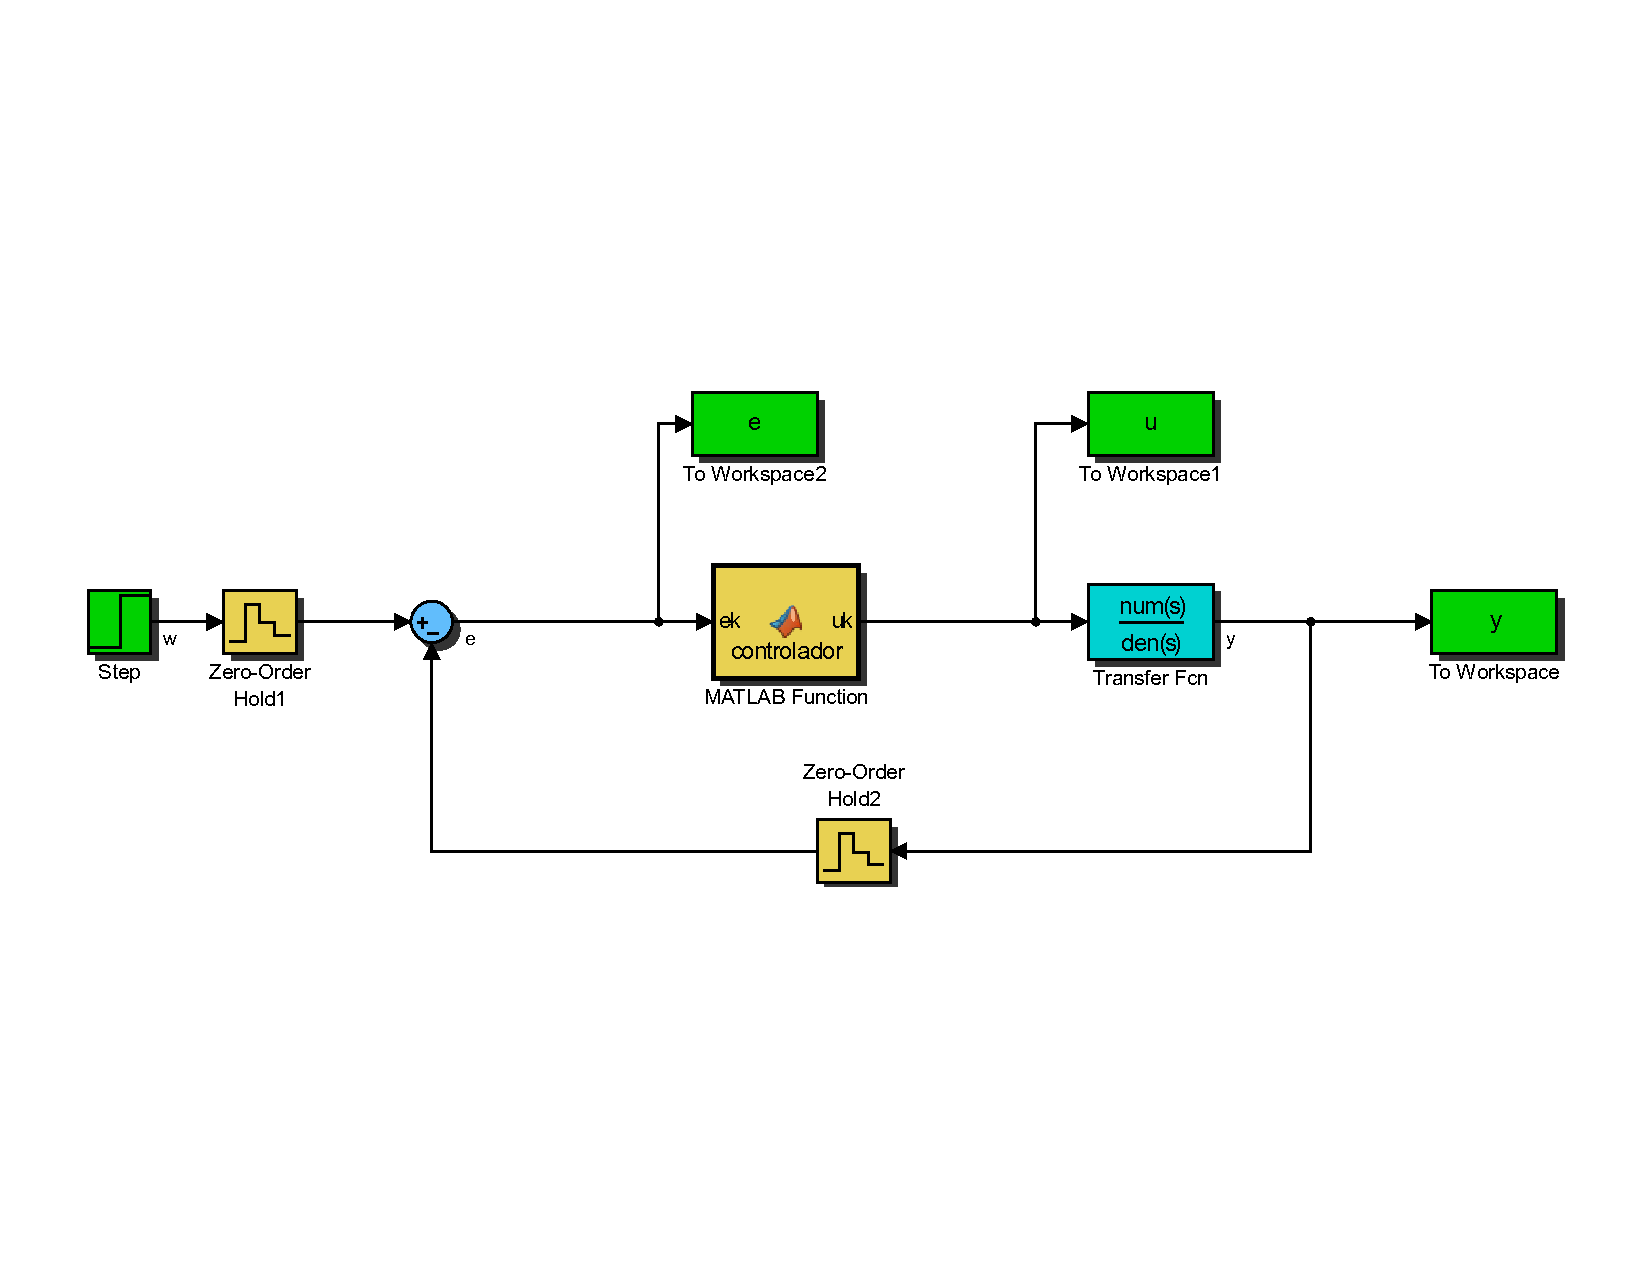
\includegraphics[width=0.6\textwidth]{./images/ex6simdiscreto.pdf}
    	\caption{Curva original e série amostrada}
    	\label{fig:ex1}
    \end{figure}
    

\section*{Dedução do exercício 7}
\label{sec:deducao7}

    O objetivo é encontrar uma função de transferência $G(z) = \frac{Y(z)}{U(z)}$ em sua respectiva função de diferenças e assim saída $y[k]$ no instante $k T_s$. Considere a função de transferência a seguir em sua forma matricial
    
        \begin{equation}
            G(z) = \frac{b^T \textbf{z}_m}{a^T \textbf{z}_n}    
            \label{eq:Gz}
        \end{equation}
    
    os quais $a \in \mathbb{R}^n$, $b \in \mathbb{R}^m$ e $\mathcal{Z}_k = \left[z^k, \cdots, 1\right]^T$. Após manipulação algébrica, $\textbf{z}_p = z^p \, \textbf{v}_p$, $\textbf{v}_p = [1, \cdots, z^{-p}]$. A fim de manter a convenção para $z^{-1}$ dada por $\textbf{w}_p =  [z^{-p}, \cdots, 1]$, $\textbf{w}_p = \textbf{J}_p \textbf{v}_p \Leftrightarrow{\textbf{v}_p = \textbf{J}_p \textbf{w}_p}$, com $\textbf{J}_p$ a matriz de permuta, descrita em (\ref{eq:exchange}).
    
        \begin{equation}
            G(z) = z^{m-n}\frac{b^T \textbf{v}_m}{a^T \textbf{v}_n} = z^{m-n} \frac{\textbf{b}^T \textbf{J}_{m+1} \textbf{w}_m}{\textbf{a}^T \textbf{J}_{n+1} \textbf{w}_n}
        \label{eq:Gv}
        \end{equation}
    
        \begin{equation}
            \textbf{J}_p = 
            \begin{bmatrix}
                0&\cdots&1\\
                \vdots & \ddots & \vdots\\
                1&\cdots&0
            \end{bmatrix}
            \label{eq:exchange}
        \end{equation}
    
    O termo $z^{m-n}$ em (\ref{eq:Gw}) deve integrar a função a fim de chegarmos à equação de diferenças. Por meio de manipulação matricial, chegamos à seguinte equação 
    
        \begin{equation}
            G(z) = \frac{\textbf{b'}^T \textbf{w}_{m'}}{\textbf{a'}^T \textbf{w}_{n'}}
            \label{eq:Gw}
        \end{equation}
    
    com $\textbf{a'} = \begin{cases} \textbf{a}\\ \begin{bmatrix} \textbf{0} \\ \textbf{J}_{n+1} \textbf{a} \end{bmatrix}_{m+1} \end{cases} \mbox{ e } \textbf{b'} = \begin{cases} \begin{bmatrix} \textbf{0}\\ \textbf{J}_{m+1} \textbf{b} \end{bmatrix}_{n+1} &, n \geq m \\ \textbf{b} &,  n < m \end{cases}$. Perceba que $n'$ e $m'$ são $\begin{cases} n + 1,& n \geq m \\ m + 1, & n < m \end{cases}$, i.e. $\forall z^p \in \textbf{w} \mbox{, } p \leq 0$. 
    
    A equação de diferenças de $G(z^{-1}) = \frac{Y(z^{-1})}{U(z^{-1})} = \frac{\textbf{b}^T \textbf{w}_{m}}{\textbf{a}^T \textbf{w}_{n}}$ é, por definição, descrita por $\textbf{a}^T \textbf{y}_{m}[k] = \textbf{b}^T \textbf{u}_{n}[k]$. Por inspeção, $a' = a$ e $b' = b$. O vetor $\textbf{y}_{n'}[k]$ pode ser escrito como $\textbf{y}_{n'}[k] = \left(\textbf{I}_{n' + 1} - \mathbf{\Delta}_{n'+1, n'+1}\right) \mathbf{y}_{n'}[k] + \mathbf{\Delta}_{n'+1, n'+1} \mathbf{y}_{n'}[k]$. A matriz $\mathbf{\Delta}_{ij}$ é definida por 
    
        \begin{equation}
          \mathbf{\Delta}_{ij} = 
          \begin{cases}
               1 & \mbox{em (i, j)}\\
               0 & \mbox{ademais}
          \end{cases}
        \end{equation}
    
    Desta forma, a equação 
    
        \begin{equation}
            \textbf{a'}^T \underbrace{\Delta_{n' + 1, n' + 1} \textbf{y}_{n'}[k]}_{\textbf{e}_{n'+1} y[k]} = \textbf{b'} \textbf{u}_{m'}[k] - \textbf{a'}^T (\textbf{I}_{n'+1} - \Delta_{n' + 1}) \textbf{y}_{n'}[k]
         \end{equation}
    
    com $\textbf{e}_{k} \in \mathbb{R}^{m'+1}$ o vetor canônico. Portanto
    
        \begin{equation}
            y[k] = \left(\textbf{a'}^T \textbf{e}_{n' + 1}\right)^{-1}\left(\textbf{b'}^T \textbf{u}_{m'}[k] - \textbf{a'}^T (\textbf{I}_{n' + 1} - \Delta_{n' + 1, n' + 1}) \textbf{y}_{n'}[k]\right)
            \label{eq:u_resumido}
        \end{equation}
    
    A equação \eqref{eq:u_resumido} tem implementação relativamente custosa por questões de requisitos de projeto. Os requisitos sã0 obter uma função \texttt{tf2diff(G, u, y)}, com \texttt{G} a função de transferência $G$, \texttt{y} os $n$ valores anteriores da saída $y$ e \texttt{u} os $m$ valores anteriores da entrada $u$ e o valor atual $u[k]$.
    
    Matematicamente, o vetor de entrada $\texttt{u} = \mathbf{u}_0^T[k] = \left[u[k - m], \cdots, u[k]\right]$ e saídas $\texttt{y} = \mathbf{y}_0^T[k] = \left[y[k - n], \cdots,\right.$ $\left.y[k - 1]\right]$. A saída $y[k]$ não existe antecipadamente como enunciado em \eqref{eq:u_resumido}. Além disso, $\dim(\texttt{y}) = n$ e $\dim(\texttt{u}) = m + 1$. Assim, reescrevemos a equação \eqref{eq:u_resumido} a fim de obter uma forma computável. Por fim
    
        \begin{equation}
            y[k] = (\textbf{a'}^T \textbf{e}_{n' + 1})^{-1}(\textbf{b'}^T \textbf{u}[k] - \textbf{a'}^T \textbf{F} \textbf{y}[k])
            \label{eq:u_programacao}
        \end{equation}
    
    com $\textbf{a'} = \begin{cases} \textbf{a}\\ \begin{bmatrix} \textbf{0} \\ \textbf{J}_{n+1} \textbf{a} \end{bmatrix}_{m+1} \end{cases} \mbox{, } \textbf{b'} = \begin{cases} \begin{bmatrix} \textbf{0}\\ \textbf{J}_{m+1} \textbf{b} \end{bmatrix}_{n+1} &\mbox{, } n \geq m \\ \textbf{b} &\mbox{, } n < m \end{cases} \mbox{ e } \textbf{F} = \begin{cases}\begin{bmatrix} \textbf{I}_{n} & \textbf{0} \\ \textbf{0} & 0 \\ \end{bmatrix}_{n+1, n} &\mbox{, } n \geq m \\ \begin{bmatrix} \textbf{0}_{m-n} & \textbf{0} \\ \textbf{0} & \textbf{I}_{n} \\ \textbf{0} & \textbf{0} \\ \end{bmatrix}_{m+1, n} & \mbox{, } n < m \end{cases}$

\section*{Exercício 7}

    O controlador PID com possibilidades de controle anti-wind-up e pólo adicional para a parte derivativa apresenta esquematicamente a seguinte estrutura:
    
        \begin{equation}
            U(s) = P(s) + I(s) + D(s)
            \label{eq:PID}
        \end{equation}
    
    com 
    
        \begin{equation}
            P(s) = K_p E(s),
            \label{eq:P}
        \end{equation},
    
        \begin{equation}
            I(s, E(s), U(s), U_{sat}(s)) = \begin{cases}
            \frac{K_p}{T_i s} E(s) & \mbox{sem anti-windup} \\
            \frac{K_p}{T_i s} E(s) - \frac{K_p}{T_t s} \left(U(s) - U_{sat}(s)\right)& \mbox{com anti-windup}
            \end{cases}
            \label{eq:I}
        \end{equation},
    
        \begin{equation}
            D(s, E(s)) = 
            \begin{cases}
                K_p T_d s E(s), & \mbox{sem filtro} \\
                K_p T_d s \frac{1}{\frac{T_d}{N}s + 1} E(s), & \mbox{com filtro} \\
            \end{cases}
            \label{eq:D}
        \end{equation}
    
    Por meio da definição de $a, f \in \{0, 1\}$, para $a$ caso haja anti-windup e $f$ para pré-filtro, reescrevemos as equações \eqref{eq:I} e \eqref{eq:D} como
    
        \begin{equation}
            I(s, E(s)) =  \frac{K_p}{T_i s} E(s) - a \frac{K_p}{T_t s} \left( U(s) - U_{sat}(s)\right)
            \label{eq:Ia}
        \end{equation},
    
        \begin{equation}
            \begin{split}
                D(s, E(s)) &= K_p T_d s E(s) \left((1-f) + f \frac{1}{\frac{T_d}{N}s + 1}\right) \\
                & = K_p T_d s E(s) + f \left(\frac{s}{\frac{T_d}{N} s + 1}  - s\right) E(s) \\
                & = K_p T_d s E(s) + f \frac{\frac{T_d}{N} s^2}{\frac{T_d}{N}s + 1} E(s)
            \end{split}
            \label{eq:Df}
        \end{equation}
    
    Ao substituirmos as expressões \eqref{eq:P}, \eqref{eq:Df}, \eqref{eq:Df}, a expressão geral \eqref{eq:PID} consequentemente segue 
    
        \begin{equation}
            U(s) = K_p \left(1 + \frac{1}{T_i s} + T_d s + f \frac{\frac{T_d}{N} s^2}{\frac{T_d}{N}s+1}\right) E(s) +  a \frac{K_p}{T_t s} U_{sat}(s) - a \frac{K_p}{T_t s} U(s)
            \label{eq:PIDaf}
        \end{equation}
    
    Perceba que para $f=0$, o termo referente ao pré-filtro é nulo e para $a = 0$, o termo anti-windup é nulo. A fim de implementá-la, a expressão segue
    
        \begin{equation}
            \begin{split}
                U(s) &= K_p \left(\frac{T_t s}{T_t s + a} + \frac{T_t s}{T_t s + a} + \frac{T_d T_t s^2}{T_t s + a} + f \frac{\frac{T_d}{N} T_t s^3}{\left(\frac{T_d T_t}{N} s^2 + \left(\frac{T_d}{N} + T_t\right) s + a\right)} \right) E(s) + \frac{a K_p}{T_t s + a} U_{sat}(s) \\
                & \coloneqq \left(P'(s) + I'(s) + D'(s) + f F(s)\right) E(s) + a W(s) U_{sat}(s)
            \end{split}
            \label{eq:PIDfull}
        \end{equation}
    
    Como já explicitado na seção \emph{\nameref{sec:deducao7}}, convertemos cada uma das expressões $P'(s)$, $I'(s)$, $D'(s)$, $F(s)$ e $F(s)$ associadas aos termos dados pela sobreposição linear \eqref{eq:PIDfull}.

\section*{Dedução dos exercícios 8 e 9}
\label{sec:deducao89}

    O objetivo dos exercícios (8) e (9) é encontrar $G(z)$ dada transformação $s = F(z)$. Em geral, as transformações aplicadas em engenharia respeitam a relação $s = \frac{c^T \mathcal{Z}}{d^T \mathcal{Z}}$, $c, d \in \mathbb{R}^2$, $\mathcal{Z}^T = [z, 1] $. Para a função de transferência dada por $G(s) = \frac{b^T \mathcal{S}_m}{a^T \mathcal{S}_n}$, tal que $\mathcal{S}_k^T = [s^k, \cdots, 1]  \, \in \, \mathbb{R}^{k+1}$, $m = \dim(b)$ e $n = \dim(a)$ e $s \in \mathbb{C}$, segue
    
    \begin{equation}
        s^i = \frac{c^T \mathcal{Z} \, c^T \, \mathcal{Z} \, \cdots \, c^T \, \mathcal{Z}}{d^T \, \mathcal{Z} \, d^T \, \mathcal{Z} \, \cdots d^T \, \mathcal{Z}} \, i \in \mathbb{N}
        \label{eq:sexpi}
    \end{equation}
    
    Por definição, $a b^T = M \,\, M \in \mathbb{R}^{2x2}$, $M = V \Lambda V^{-1}$, $\forall M \in \mathbb{R}^{n \times n}$, com $V$ a matriz direita de autovetores de $M$ e $\Lambda$ a matriz de autovalores de $M$, diagonal por definição. Além disso, $f(M) = V f(\Lambda) V^{-1}$. Em especial, $M^i = V \Lambda^i V^{-1}$. Assim, a equação (\ref{eq:sexpi}) reduz-se a:
    
    \begin{equation}
        s^i = \frac{c^T V_c \Lambda_c^{i-1} V_c^{-1} \mathcal{Z}}{d^T V_d \Lambda_d^{i-1} V_d^{-1} \mathcal{Z}}
    \end{equation}
    
    Perceba que o expoente de $\Lambda$ deve ser $k - 1$ por questão construtiva. Além disso, para uma matriz $\Lambda_c$ e $\Lambda$ arbitrárias, para $k = 0$, $\Lambda_c^{-1} = \Lambda_c^{+}$. Construtivamente
    
    \begin{equation}
        \mathcal{S}_k^T = \left[\frac{c^T V_c \Lambda_c^{k-1} V_c^{-1} \mathcal{Z}}{d^T V_d \Lambda_d^{k-1} V_d^{-1} \mathcal{Z}}, \cdots, \frac{c^T V_c \Lambda_c^{k-1} V_c^{-1} \mathcal{Z}}{d^T V_d \Lambda_d^{k-1} V_d^{-1} \mathcal{Z}}\right]
    \end{equation}
    
    Deste modo, a função convertida pela função de transformação $s = \frac{c^T \mathcal{Z}}{d^T \mathcal{Z}}$ é dada por
    
    \begin{equation}
        G(z) = \frac{b^T \mathcal{S}_m}{c^t \mathcal{S}_n}    
    \end{equation}
    
    \begin{equation}
        \mathcal{S}_k^T = \left[\frac{c^T V_c \Lambda_c^{k-1} V_c^{-1} \mathcal{Z}}{d^T V_d \Lambda_d^{k-1} V_d^{-1} \mathcal{Z}}, \cdots, \frac{c^T V_c \Lambda_c^{k-1} V_c^{-1} \mathcal{Z}}{d^T V_d \Lambda_d^{k-1} V_d^{-1} \mathcal{Z}}\right]
    \end{equation}

\section*{Exercício 8}

    A transformação para trás tem parâmetros $c^T = [1, -1]$ e $d^T = [T_s, 0]$ e a transformação para frente $c^T = [1, -1]$ e $d^T = [0, T_s]$. A implementação em MatLab encontra-se em anexo.

\section*{Exercício 9}
\label{ex:ex9}

    A transformação de Tustin tem parâmetros $c^T = [2, 2]$ e $d^T = [T_s, -T_s]$. A implementação em MatLab encontra-se em anexo.

\section*{Exercício 10}

\subsection*{Solução 1}

    Seja $P(z) = 1 + K G(z)$, o polinômio característico de $G(z)$ em malha fechada, para $K \in \mathbb{R}^*_{+}$ e $W$ o lugar geométrico das raízes do polinômio. O polinômio apresenta $N-1$ pólos em $z = 0$ e 1 pólo em $z = 1$. No caso em estudo, $G(z) = \frac{1}{z^{N} - z^{N-1}}$.
    
    Seja $\forall N \in \mathbb{N}^*\backslash{\{1\}}$, $S \in W$, $S = \{z \in \mathbb{C}, \omega \in \mathbb{R}, \sigma \in [0, 1] \,\, | \,\, z = (\omega, \sigma)\}$. Assim, por inspeção geométrica, $\inf K = 0$ para assegurar estabilidade. Para K crescente em $M = W \backslash {S}$, as ramificações resultantes divergem da origem e passam pela circunferência unitária i.e. $\exists K$, $K_{max} = \sup K$. e, assim, $0 \leq K \leq K_{max}$
    
    Para o limite de estabilidade i.e. $|z| \stackrel{!}{=} 1$ ou $z = e^{j \theta}$, tal que a malha fechada do sistema seja estável, tem-se que
    
        \begin{equation}
            P(z = e^{j \theta}) \coloneqq 0 = e^{j (N-1) \theta} - e^{j N \theta}
            \label{eq:Pz}
        \end{equation}
    
    Seja a transformação de Euler $e^{j \theta} = \cos{\theta} + j \sin{\theta}$ e as relações trigonométricas $\cos{a} - \cos{b} = -2 \sin{a+b} \sin{\frac{a-b}{2}}$ e $\sin{a} - \sin{b} = 2 \sin{\frac{a-b}{2}} \cos{\frac{a+b}{2}}$, para $K \in \mathbb{R}$, a equação (\ref{eq:Pz}) torna-se:
    
        \begin{subequations}
            \begin{equation}
                K = -2 \sin\left((2N - 1) \frac{\theta}{2}\right) \sin\left(- \frac{\theta}{2}\right)
            \end{equation}
            \begin{equation}
                0 =  2 \cos\left((2N - 1) \frac{\theta}{2}\right) \sin\left(-\frac{\theta}{2}\right)
            \label{eq:imagP}
            \end{equation}
        \end{subequations}
    
    Da equação (\ref{eq:imagP}), $S = S_1 \cup S_2$, $S_1 = $ $ \left\{\theta \in [0, 2 \pi] \,\, \Bigr| \,\, \theta = 0\right\}$, $S_2 = \left\{k \in \mathbb{Z}, \,\, \theta \in [0, 2 \pi] \,\, \Bigr| \,\, \theta = \frac{\pi}{2N - 1} + \frac{2 \pi}{2N - 1} k\right\}$. Para $S_1$, $L_1 = \left\{K \in \mathbb{N}^* \,\, \Bigr| \,\, K = 0\right\}$. Para $S_2$, $L_2 = \left\{K \in \mathbb{N}^*, k \in \mathbb{Z} \,\, \Bigr| \,\, 2 \, \sin\left(\frac{\pi}{2N-1} + \frac{2 \pi}{2N-1} k\right)\right\}$. Por verificação, $k \in [0, 2N -1]$, e a função seno no intervalo dado é estritamente crescente. Assim, 
    
        \begin{equation}
            K_{max} = K(k) = K(2N - 1) = 2 \sin\left(\frac{\pi}{(2N - 1) 2}\right)
        \end{equation}
    
    Por fim, como $\sin(\frac{\theta}{2}) = \sqrt{\frac{1 - \cos{\theta}}{2}}$ Assim,
    
        \begin{equation}
            0 \leq K \leq \sqrt{2 \left(1 - \cos\left(\frac{\pi}{2N - 1}\right)\right)} \hspace{10pt} \blacksquare
        \end{equation}

\subsection*{Solução 2}

    Seja $P(z) = 1 + K G(z)$, o polinômio característico de $G(z)$ em malha fechada, para $K \in \mathbb{R}^*_{+}$ e $W$ o lugar geométrico das raízes do polinômio. O polinômio apresenta $N-1$ pólos em $z = 0$ e 1 pólo em $z = 1$. No caso em estudo, $G(z) = \frac{1}{z^{N} - z^{N-1}}$.  Assim $K = z^{N - 1} - z^N$. Para o limite de estabilidade $z = e^{j\theta} = \cos{\theta} + j \sin{\theta}$, tem-se que:
    
    \begin{equation}
        \begin{split}
            K(z) & = e^{j N \theta} \left(1 - e^{-j \theta}\right) \\
             & = e^{j N \theta} \left(1 - e^{-j \theta}\right)  \frac{e^{\frac{j\theta}{2}}}{e^{\frac{j\theta}{2}}} \frac{2j}{2j} \\
             & = 2 j e^{\frac{j (2N - 1) \theta}{2}} \underbrace{\left(\frac{e^{\frac{j \theta}{2}} - e^{\frac{- j \theta}{2}}}{2 j}\right)}_{\sin(\frac{\theta}{2})} \\
             & = -2 j e^{j \frac{(2N - 1) \theta}{2}} \sin{\frac{\theta}{2}}
        \end{split}    
    \end{equation}
    
    Como $K \in \mathbb{R^*_+}$, temos que 
    
    \begin{subequations}
        \begin{equation}
            \begin{split}
            K & \coloneqq |2| . |e^{j \frac{(2N - 1)\theta}{2}}| . |\sin(\frac{\theta}{2})| |\frac{1}{j}| \\
            & = 2 \sin{\left(\frac{\theta}{2}\right)}
            \end{split}
            \label{eq:modulo}
            \end{equation}
            \begin{equation}
            0 \coloneqq \angle(2) + \angle\left(e^{\frac{(2N + 1)\theta}{2}}\right) + \angle\left(\sin\left(\frac{\theta}{2}\right)\right) + \angle(\left(\frac{1}{j}\right)) \\
             = \frac{(2N - 1)}{2} \theta - \frac{\pi}{2}
            \label{eq:argumento}
        \end{equation}
    \end{subequations}
    
    Por \eqref{eq:argumento}, obtemos que $\theta = \frac{\pi}{2N - 1}$. Ao substituir em \eqref{eq:modulo}, temos que $K = 2 \sin\left(\frac{\pi}{2 (2N - 1)}\right)$. Como $sin\left(\frac{\theta}{2}\right) = \sqrt{\frac{1 -\cos(\theta)}{2}}$, por fim
    
    \begin{equation}
        0 \leq K \leq \sqrt{2 \left(1 - \cos\left(\frac{\pi}{2N - 1}\right)\right)} \hspace{10pt} \blacksquare
    \end{equation}

\newpage

\section*{Scripts}
    \subsection*{syms2tfz.m}
    \label{subsec:syms2tfz}
    \lstinputlisting[language=Matlab, caption=Conversão de simbólico fracionário em função de transferência discreta]{code/syms2tfz.m}
    
    \subsection*{s2z.m}
    \label{subsec:s2z}
    \lstinputlisting[language=Matlab, caption=Conversão de função de transferência por transformação $T(z)$]{code/s2z.m}
    
    \subsection*{backward.m}
    \label{subsec:backward}
    \lstinputlisting[language=Matlab, caption=Transformação de conversão para trás]{code/backward.m}
    
    \subsection*{forward.m}
    \label{subsec:forward}
    \lstinputlisting[language=Matlab, caption=Transformação de conversão para frente]{code/forward.m}
    
    \subsection*{tustin\_prop.m}
    \label{subsec:tustin}
    \lstinputlisting[language=Matlab, caption=Transformação de conversão tustin própria]{code/tustin_prop.m}

\end{document}